%------------------------------%
\chapter[Modeling Social Intelligence via Norms]{Modeling Social Intelligence via Norms to Engineer Privacy-Aware Personal Agents}
\label{chap:arnor}
%------------------------------%

This chapter describes \frameworkA, our methodology to model social
intelligence in personal agents, and its empirical evaluation via a
developer study and simulation experiments. It is based on a
paper ``Arnor: Modeling Social Intelligence via Norms to Engineer
Privacy-Aware Personal Agents'' that appears in \emph{Proceedings of the
16th International Conference on Autonomous Agents and Multiagent
Systems (AAMAS)}.

\section{Introduction}
\label{sec:arnor-intro}

Our actions and interactions in a society are not driven solely by
individual needs. Instead, we adapt our behavior considering the needs
of others, e.g., by being courteous and lending a helping hand. Such
acts, even if inconvenient at times, deliver a pleasant social
experience.

Privacy encompasses both social and technical aspects. However, most of
the traditional works have approached privacy from a technical
standpoint. We tackle the science of privacy from a sociotechnical
viewpoint \citep{Kafali-IS16-Revani,WWW-16:IOSE}.

Consider a society in which an agent acts and interacts on behalf of a
\emph{stakeholder} (human user). Our objective is to engineer the agents
such that they deliver a \emph{social experience} relative to that
society, as opposed to individual user experiences. We refer to an agent
delivering a social experience as a \emph{socially intelligent personal
agent} (SIPA). The \emph{primary} stakeholder of a SIPA is the user who
directly interacts with the SIPA, and on whose behalf the SIPA acts and
interacts. A \emph{secondary} stakeholder of a SIPA may not directly
interact with the SIPA, but the SIPA's actions affect the secondary
stakeholder.

To understand the nuances in modeling social intelligence in SIPAs, 
let us revisit the example in Chapter~\ref{chap:intro}. 

\begin{example} \label{ex:ringer-meeting} Consider a ringer manager as a
SIPA installed on Alice's phone. The ringer manager decides appropriate
ringer modes (e.g., loud or silent) for incoming calls. Alice is the
ringer manager's primary stakeholder. Bob, Alice's friend, calls her
when Charlie and Dave, Alice's coworkers, are in her vicinity. Bob,
Charlie, and Dave are the ringer manager's secondary stakeholders.
\end{example}


We define social experience as the collective experience a SIPA delivers
to each of its primary and secondary stakeholders. Respecting
stakeholders' privacy is an important aspect of delivering social
experience.

\begin{example} \label{ex:ringer-implications} Bob calls Alice when she
is in an important meeting with Charlie and Dave. \end{example}

In Example~\ref{ex:ringer-implications}, should Alice's phone ring loud
during the meeting, privacy implications may follow
\citep{solove-2006-taxonomy,Murukannaiah-IC16-Engineering}. A loud ring
\emph{intrudes} upon Alice's and other meeting attendees' privacy in
that the call violates their reasonable expectation to be left alone.
Further, Alice may receive nasty looks from other attendees
(\emph{disapprobation}). If Alice answers the call, those overhearing
Alice and Bob's conversation can gain knowledge about her and her
interlocutor (\emph{information leak}).

\begin{example} \label{ex:ringer-accident} Alice is in a meeting with
Charlie and Dave. Bob is in a car accident and calls Alice for
assistance. Bob's ringer manager communicates the urgency to Alice's
ringer manager, which then sets her phone to ring loud. It also notifies
Charlie and Dave about the situation. \end{example}

Should Alice's phone stay silent for Bob's urgent call, Bob's trust for
Alice may reduce, affecting their social relationship. Instead, if the
phone rings loud and Alice communicates a rationale to Dave and Charlie,
presumably, they would not frown at her.

These examples demonstrate the nontrivial decisions a SIPA must make and
the implications those decisions have on the stakeholders' social
experience and privacy. These nuances prompt us to investigate the
research question:

\begin{description}[leftmargin=1em] \item[RQ.] How can we engineer a
SIPA such that it delivers a social experience but respects its
stakeholders' privacy? \end{description}

%
Three key challenges in engineering a SIPA to deliver a social experience are understanding
\begin{enumerate*}[label=(\arabic*)]
\item what constitutes social experience;
\item how a SIPA's actions influence the social experience and privacy for each stakeholder; and
\item how a SIPA's actions evolve when it is put to use in a 
variety of social contexts.
\end{enumerate*}

Existing agent-oriented software engineering (AOSE) methods provide a
good starting point for addressing the first challenge. For example,
Tropos \citep{Bresciani-JAAMAS04-Tropos} actor models and Gaia
\citep{Wooldridge-2000-Gaia} interaction models capture stakeholders and
coarse dependencies between them. However, these methods provide little
guidance on capturing how an agent's actions and interactions influence
each stakeholder involved (second challenge). Also, these methods
provide design-time constructs to model an agent, but fall short in
modeling social interactions that support agents to adapt to evolving
social contexts at run time (third challenge). Our formulation contrasts
with Tropos where the stakeholders are characterized by their goals, as
in caller, callee, and neighbor, but a single perspective is taken in
the actor produced. We consider multiple perspectives where each agent
corresponds to one user and has its loyalty to that user.

Norms have been widely studied with several works addressing norm
conflicts, compliance, and emergence via either simulation or
formalization \citep{Alechina+16:monitoring,Criado-IJCAI16-Selective}.
\Citet{vanRiemsdijk-AAMAS15-SAEP} argue for a personal
agent's need to explicitly represent norms. Social norms inform SIPAs
about a set of reasonable actions in a social context. Norm compliance
in a social context is achieved either by
%
\begin{enumerate*}[label=(\arabic*)]
\item establishment of norms, where SIPAs are made aware of norms by 
direct communication, or
\item via (positive and negative) sanctions, where SIPAs learn norms in 
the form of appropriate actions in a social context 
\citep{Andrighetto-2013-PunishVoice}.
\end{enumerate*}
%
Also, a SIPA's decision rationale for its action influences
how other stakeholders perceive satisfaction or violation of a norm, and 
the nature of sanctions that they apply. 

\subsubsection*{Contribution} 
To address the aforesaid challenges, we propose \frameworkA, a systematic 
method enabling the development of privacy-aware socially intelligent personal 
agents via social constructs.  \frameworkA facilitates agent developers in modeling
stakeholders' social expectations and, how an agent's actions influence 
those expectations, thereby enabling SIPAs that deliver a rich
social experience.  
\frameworkA employs Singh's \citeyearpar{Singh-2013-Norms} model of (social)
norms to capture social requirements, and incorporates argumentation
constructs \citep{BenchCapon-2007-Argumentation+AI} for
sharing a decision rationale.

Testing a SIPA's adaptability in all possible social contexts would be infeasible. 
To overcome this challenge, \frameworkA incorporates a SIPA simulation testbed. 
Seeded with crowdsourced data, \frameworkA's testbed enables designers to test a
SIPA's runtime adaptability.
We rigorously evaluate \frameworkA via two studies:
\begin{enumerate*}[label=(\arabic*)]
\item a multiphase developer study in which developers engineer a SIPA,
and
\item a set of adaptability studies in which we simulate the
adaptability of SIPAs developed in the first study in a variety of
social contexts. \end{enumerate*}

\subsubsection*{Novelty}
\frameworkA goes beyond existing AOSE methods by assisting
developers to incorporate social norms and reason about how those norms
influence social experience. In spirit, \frameworkA is a hybrid method in
that it addresses the problem of engineering SIPAs combining top-down (via
modeling) and bottom-up (via experience or social learning
\citep{Sen-IJCAI07-NormEmergence}) styles.\\

Section~\ref{sec:arnor-preliminaries} briefly describes the background
works on which we build. Section~\ref{sec:arnor-framework} describes
\frameworkA in detail. Section~\ref{sec:arnor-experiments} describes our
developer and simulation studies, and Section~\ref{sec:arnor-result}
presents our results and discusses threats to validity.
Section~\ref{sec:arnor-related} discusses related works and
Section~\ref{sec:arnor-discussion} concludes with important future
directions.

\section{Background}
\label{sec:arnor-preliminaries}

\frameworkA builds on the AOSE methods of Tropos and Xipho, and on the 
constructs of social norms and sanctions.

\subsection{Tropos and Xipho}
\label{subsec:background}

Tropos \citep{Bresciani-JAAMAS04-Tropos} is an end-to-end AOSE
methodology spanning requirements modeling, design, and implementation.
Tropos provides systematic steps to model and refine an application to
be developed via high-level abstractions.

We adopt the following Tropos abstractions. An \emph{actor} is a social,
physical, or a software agent. An actor has \emph{goals} (strategic
interests) and \emph{plans} (means of achieving a goal) within a
system. Further, an actor's goals can be \emph{hard} (having a specific
satisfaction condition) or \emph{soft} (not have a specific satisfaction 
condition). A \emph{belief} is an actor's perspective of the environment and a
\emph{resource} is a physical or information entity. An actor may have
\emph{dependencies} with other actors to satisfy goals, execute plans,
or acquire resources.

Figures~\ref{fig:xipho-ringer-as-is} shows a Tropos system-as-is model
(the as-is model captures the setting in which the agent to be
developed, e.g., the ringer manager, operates). This model identifies the
stakeholders and dependencies between them as well as the goals and
plans of the stakeholders.

\begin{figure}[!htb] \centering
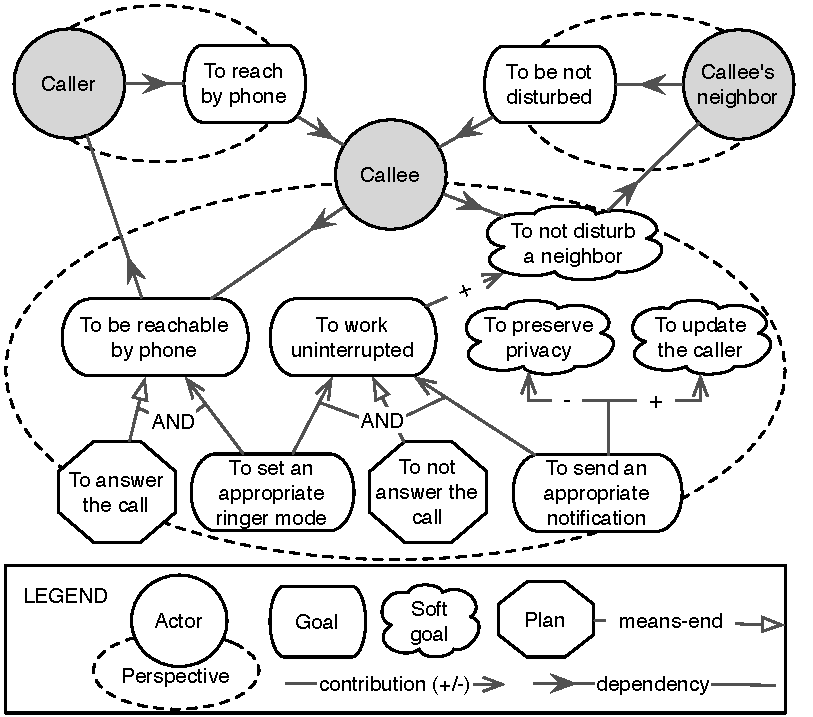
\includegraphics[angle=0,width={0.60\columnwidth}]{Chapter-3/fig/ringer-manager-tropos-actor-model.pdf}
\caption[A Tropos model of the ringer manager]{A Tropos system-as-is model of the ringer manager, expanding the callee's perspective \protect\citep{Murukannaiah-AAMAS14-Xipho}.}
\label{fig:xipho-ringer-as-is} \end{figure}

Xipho \citep{Murukannaiah-AAMAS14-Xipho} extends Tropos to engineer
personal agents. Xipho introduces \emph{context} as a high-level
abstraction and treats an actor's goals, plans, and dependencies as
inherently contextual. Xipho enables a developer to tailor a generic
model of context to a specific application scenario via systematic steps
through distinct development phases.

\subsection{Norms and Sanctions}

A norm as understood here \citep{Singh-2013-Norms} is directed from a
subject to an object and is constructed as a conditional relationship
involving an antecedent (which brings the norm in force) and a
consequent (which brings the norm to satisfaction or violation). This
representation yields clarity on who is accountable to whom. A norm can
be formalized as:
%
\begin{center}
$\N(\fsc{subject},\fsc{object}, antecedent, consequent)$
\end{center}

We employ the following types of norms in our approach. 
\begin{itemize}

\item A \emph{commitment} ($\C$) means that its subject commits to its
object to ensure the consequent if the antecedent holds. An example
commitment is that, in a meeting room, the participants may be committed
to each other to keep their phones silent: $\C$($\fsc{phone-user}$,
$\fsc{coworker}$, $\text{place}=meeting$, $\text{ring}=silent$).

\item A \emph{prohibition} means that its subject is forbidden by its
object from bringing about the consequent if the antecedent holds. An
example prohibition ($\Pro$) is that, in an examination hall, the
students may be prohibited by a proctor from answering phone calls:
$\Pro$($\fsc{phone-user}$, $\fsc{proctor}$, $\text{place}=examination$,
$\text{ring}=silent$).

\item A \emph{sanction} specifies the consequences its subject faces
from its object for satisfying or violating another norm, such as a
commitment or a prohibition. A sanction can be positive, negative, or
neutral \citep{Nardin-KER16-Classifying}. A sanction may be in the form
of ``feedback,'' e.g., a smile or a scowl, from one user to another. An
example sanction ($\San$) is that, in a meeting, if a participant's
phone rings loud, he or she receives a scowl from other meeting
participants: $\San$($\fsc{phone-user}$, $\fsc{coworker}$,
$\text{place}=meeting \land ring=loud$, $\text{feedback}=scowl$).

\end{itemize} 

\section{\frameworkA}
\label{sec:arnor-framework}

\frameworkA is a four-step method build on social constructs to systematically model the social 
experience provided by a SIPA. \frameworkA's steps include modeling of: 
\begin{enumerate*}[label=(\arabic*)]
\item goals, 
\item environmental contexts,
\item social expectations, and 
\item social experience. 
\end{enumerate*}
Figure~\ref{fig:arnor-model} shows a conceptual model of 
\frameworkA.  Table~\ref{tab:arnor-steps} provides an overview. 


\begin{figure}[!htb] 
\centering
% 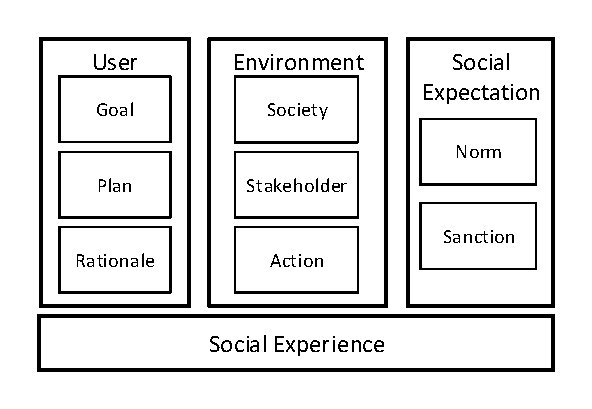
\includegraphics[angle=0,width={0.60\columnwidth}]{Chapter-3/fig/model}
\resizebox{0.6\columnwidth}{!}{

\begin{tikzpicture}[auto, node distance=2cm,>=latex',font=\small]
\tikzset{block/.style = {draw, rectangle, minimum height=2em, 
  minimum width=4em}}
\pgfdeclarelayer{background}
\pgfdeclarelayer{foreground}
\pgfsetlayers{background,main,foreground}

  \begin{pgfonlayer}{foreground}
    \node[block, fill=blue!10, minimum width = 2.0cm] (goal){Goal};
    \node[block, fill=blue!10, minimum width = 2.0cm, node distance=.8cm, below of=goal] 
      (plan){Plan};
    \node[block, fill=blue!10, minimum width = 2.0cm, node distance=.8cm, below of=plan] 
      (rationale){Rationale};


    \node[block, fill=blue!10, minimum width = 2.0cm, node distance=2.5cm, right of=goal] 
      (society){Society};
    \node[block, fill=blue!10, minimum width = 2.0cm, node distance=.8cm, below of=society] 
      (stakeholder){Stakeholder};
    \node[block, fill=blue!10, minimum width = 2.0cm, node distance=.8cm, below of=stakeholder] 
      (action){Action};
  
    \node[block, fill=blue!10, minimum width = 2.0cm, node distance=2.5cm, right of=society] 
      (norm){Norm};
    \node[block, fill=blue!10, minimum width = 2.0cm, node distance=.8cm, below of=norm] 
      (sanction){Sanction};
  
  \end{pgfonlayer}
  
  \node[fit= (goal) (plan) (rationale), inner sep=.5em, align=center, 
    minimum height = 3.6cm, minimum width = 2cm, yshift=.4cm,
    fill=blue!50!black, rounded corners=.15cm,
    label={[yshift=-.7cm, align=center, text=white]
   User}](user){};

  \node[fit= (society) (stakeholder) (action), right of=user,
    node distance=2.5cm,
    inner sep=.5em, align=center, 
    minimum height = 3.6cm, minimum width = 2cm,
    fill=blue!50!black, rounded corners=.15cm,
    label={[yshift=-.7cm, align=center, text=white]Environment}]
    (environment){};
  
  \node[fit= (norm) (sanction), right of=environment,
    node distance=2.5cm,
    inner sep=.5em, align=center, 
    minimum height = 3.6cm, minimum width = 2cm,
    fill=blue!50!black, rounded corners=.15cm,
    label={[yshift=-1.0cm, align=center, text=white]Social\\Expectation}]
    (socialexpectation){};

  \node[node distance=2.2cm, below of=environment, minimum height=.7cm,
    fill=blue!50!black, rounded corners=.15cm,
    text=white, minimum width=7.4cm] 
    (socialexperience){Social Experience};

  \begin{pgfonlayer}{background}
  \node[fit= (user) (environment) (socialexpectation)
    (socialexperience), rounded corners=.25cm, fill=gray!20,
    inner sep=.5em, align=center, minimum height = 4.8cm, minimum width = 2cm]
    (arnor){};
  \end{pgfonlayer}

\end{tikzpicture}

}
\caption[\frameworkA 's conceptual model schematically]{\frameworkA 's conceptual model schematically.}
\label{fig:arnor-model} 
\end{figure}

% Splitting table caption and heading across multiple pages: https://tex.stackexchange.com/questions/383898/how-to-split-long-table-in-multiple-pages
\clearpage
%\begin{table}[!htb]
\begin{longtable}{@{}p{2.2cm}p{5cm}p{7.5cm}@{}}
%\centering
\caption[Overview of \frameworkA tasks]{Overview of \frameworkA tasks and examples to engineer a SIPA.}
\label{tab:arnor-steps}\\
\toprule
\fbf{Step} & \fbf{\frameworkA Task} & \fbf{Example} \\\midrule

\endfirsthead
\caption[Overview of \frameworkA tasks]{Overview of \frameworkA tasks and examples to engineer a SIPA (continued).}\\
\toprule
\fbf{Step} & \fbf{\frameworkA Task} & \fbf{Example} \\\midrule

\endhead
    \midrule
    \multicolumn{3}{r}{\footnotesize\itshape Continue on the next page}
\endfoot
    \bottomrule
\endlastfoot

\multirow{1}{2.2cm}{Goal Modeling}& Identify all actors &   
Alice, Bob, Charlie, Dave, Erin, and strangers in the theater\\

& Abstract actors as primary and secondary stakeholders, as appropriate & Phone user is a primary stakeholder; friend, coworker, stranger in the vicinity of phone users are secondary stakeholders\\

& Identify goals of each actor & Phone user's goals \fsl{to be tele-reachable}, and \fsl{to be not disturbed} \\

& Identify all actions, and abstract them as appropriate &  \fsl{Phone users do not answer phone calls during meetings}; \fsl{phone users answers 
their coworkers' urgent phone calls}\\

& Identify plans for abstract actions & \fsl{Set ringer mode as loud} 
for the action \fsl{phone user answers a phone call} \\

& Associate goals with plans & Phone user's goal of \fsl{tele-reachable} 
can be realized by the plan of \fsl{setting ringer mode as loud}\\
\midrule

\multirow{1}{2.2cm}{Context Modeling} & Identify the contexts in which 
each actor's goals and plans are relevant 
	& Coworker's goal \fsl{to be not disturbed} is relevant in the \fsl{meeting} context\\
& Identify conflicting goals (and inconsistent plans) & 
Phone user's goal of \fsl{tele-reachable} conflicts with the goal \fsl{to not disturb neighbors} in the \fsl{meeting} context
\\
\midrule

\multirow{1}{2.2cm}{Social Expectation Modeling} & Identify norms relevant 
to social and privacy expectations & \fsl{The phone user is committed to
    answering urgent phone calls from family}
    \\
 & Identify possible conflicts between norms & \fsl{Phone user's commitment toward friend to answer phone calls} conflicts with
 \fsl{phone user's commitment to keep phone on silent during meeting}\\
 & Resolve conflicts by capturing contextual preferences between norms & 
   In the \fsl{meeting} context, prefer \fsl{phone user's commitment to keep phone on silent during meeting} over \fsl{phone user's commitment toward friend to answer phone calls}
   \\

\midrule
\multirow{1}{2.2cm}{Social Experience Modeling} & Identify effects of 
stakeholders' actions on social expectations & A norm that is consistently being violated, e.g., \fsl{phone users always answering calls during meeting}\\
& Promote actions that enhance social experience & 
\\

\bottomrule
\end{longtable}
%\end{table}

\subsection{Goal Modeling}

For a SIPA to provide a social experience, it needs to be aware of
the associated stakeholders, their goals and relevant plans. Goal
modeling in \frameworkA uses Tropos constructs to elicit stakeholders,
their goals, and relevant plans.

\begin{description}[leftmargin=1em]
\item[A stakeholder] is a user that participates in a society and 
interacts with or is affected by the SIPA.  \emph{Primary} stakeholders 
are the users that interact directly with the SIPA.  \emph{Secondary} 
stakeholders do not have direct interaction with the SIPA, but are 
affected by its interactions with the primary stakeholder.  

\item[A goal] is a set of states of the environment that are 
preferred by the stakeholders. 

\item[A plan] is a sequence of actions that can bring about a state in
which a stakeholder's goal is satisfied. The SIPA acts on behalf of the
stakeholders or assists stakeholders in bringing their goals.

\end{description}

Stakeholders in \frameworkA map to actors in Tropos or Xipho.
Whereas Tropos and Xipho explicitly relate actors to the users that
have goals, \frameworkA forces designers to additionally identify (secondary)
stakeholders that do not necessarily have a goal, but are affected by
the plans that (primary) stakeholders execute to achieve their
goals. Capturing secondary stakeholders is necessary to providing a 
social experience. A stakeholder may adopt different roles.

Following Table~\ref{tab:arnor-steps}, we create the goal
model for the ringer manager SIPA described in Examples~\ref{ex:ringer-meeting}--\ref{ex:ringer-accident} and Figure~\ref{fig:xipho-ringer-as-is}.

\begin{description}[leftmargin=1em]
  
  \item[Primary stakeholder.] Alice, the phone user (S$_1$). 

\item[Secondary stakeholders.] Bob (Alice's friend, S$_2$), Charlie and
Dave (Alice's coworkers, S$_3$ and S$_4$), Erin (Alice's mother, S$_5$)
and strangers (those in the theater who are in Alice's vicinity when
the ringer manager SIPA is in use, S$_6$). Here Bob, Charlie, Dave and Erin
could assume the roles of caller and neighbors in different contexts.
Note that, although the ringer manager SIPA includes only one primary
stakeholder, other settings could involve multiple primary stakeholders.

\item[Goals.] The phone user's goals are to be
tele-reachable (G$_1$), to notify caller if not reachable (G$_2$), to
work uninterrupted (G$_3$), and to avoid annoying
neighbors (G$_4$). Bob, Alice's friend has goals to (1) tele-reach Alice
(corresponds to G$_1$), and (2) be notified if Alice is not reachable
(corresponds to G$_2$). Charlie and Dave's goals are to not be disturbed
at work by anyone (same as G$_4$). Erin's mother has the same goals as
Bob. Strangers in Alice's vicinity share the same goal as Charlie and
Dave. When Charlie and Dave assume the caller role, they share Bob and 
Erin's goal of tele-reaching Alice.
  
\item[Actions.] Alice, the phone user, can answer a call if she is
available, or can notify the caller otherwise. She could
decide not to answer calls if she does not want to be disturbed or does
not want to annoy her neighbors. Based on Alice's actions, Bob, Charlie,
Dave, Erin, and other stakeholders act. For example, if Alice answers
Bob's or Erin's call, they could give Alice a positive feedback. In social
expectation modeling, we capture these feedback actions as sanctions. 

\item[Plans.] The plan corresponding to the \fsl{answer call} action is to
\fsl{set ringer mode on loud} (P$_1$). The other plans could be to
\fsl{set ringer mode on vibrate} (P$_2$) or \fsl{set ringer mode on
silent} (P$_3$).

\item[Goal-plan association.] The plan of setting the ringer on
loud promotes the phone user's goal of being tele-reachable, and
caller's goal of tele-reaching the callee. The plan of setting the
ringer on silent promotes the phone user's goal to work
uninterrupted, and the neighbors' goal of not being disturbed.
\end{description}

\subsection{Social Context Modeling}

Context modeling includes identifying social contexts in which the
stakeholders of a SIPA interact. The social context could include the
place where the interaction occurs, attributes of the place, neighbors
in the vicinity, the social relationship between primary and secondary
stakeholders, the activities the stakeholders are involved in, and so
on. The social context is decisive in identifying the goals to be
brought about or plans to be executed in case of conflicts.

Some of the contexts associated with goals, G$_1$--G$_4$, and plans,
P$_1$--P$_3$, are based on stakeholders' locations (meeting or theater),
social relationship (colleagues, friends or family), reason
associated with a phone call (urgent phone call or a casual phone
call), and so on.

Goal G$_1$ of being tele-reachable conflicts with goals
G$_3$ and G$_4$ for both the meeting and theater scenarios.
In these scenarios, the SIPA must rely on social
contexts to determine which goal to accomplish. Potentially,
where multiple plans may help realize the same goals. For example, in a
library, both the \fsl{phone on silent} plan and \fsl{phone on vibrate}
plans serve the goal of not disturbing one's neighbors. The SIPA
relies on social context to choose between multiple plans. 
%Conflicts are further handled in social expectation modeling and
%social experience modeling.
  
\subsection{Social Expectation Modeling}

Social expectations including the privacy ones influence the
stakeholders' goals and plans. We model these expectations between
stakeholders in terms of social norms and sanctions. The social norms of
a society regulate how stakeholders act and conduct themselves. Some
norms could be local to a stakeholder, for example, one's commitment
toward family members to always answer their phone calls, and some norms
could be specific to a social context, for example, in the context of a
meeting, a phone user is committed to keep his or her phone silent.

We express social expectations for the ringer manager SIPA via norms,
sanctions and conflicts.
\begin{description}[leftmargin=1em]
\item[Norms.] We identify the following norms.
  \begin{itemize}[leftmargin=1em]
  \item A phone user is committed to answering phone calls from
  callers. This commitment is satisfied by the plan of setting the 
  ringer mode on loud.

  $C_{caller}$: $\C(\fsc{phone-user},\fsc{caller}, \text{call}, \text{ring}=\textit{loud})$

  \item A phone user is committed to notifying the caller if he or she does
  not answer. The commitment is satisfied by the plan of setting the
  ringer mode on silent and sending a notification to the caller.
  
  $C_{notify}$: $\C(\fsc{phone-user},\fsc{caller}, \text{call},\\ 
  \text{ring}= \textit{silent}   \land \textit{notify})$
    
  \item A phone user is committed to coworkers to not let the phone ring 
  during meetings.
  This commitment is satisfied by the plan of setting the ringer mode on 
  silent or vibrate. 

  $C_{meeting}$: $\C(\fsc{phone-user},\fsc{coworkers}, \text{call},\\ 
  \text{ring}= \textit{silent} \lor \text{ring} = \textit{vibrate})$
  \end{itemize}
  
\item[Sanctions.] The associated sanctions are as below: 
  \begin{itemize}[leftmargin=1em]
  \item A phone user is (negatively) sanctioned by coworkers for 
  answering a phone call during a meeting. 
  
    $S_{meeting}$: $\C(\fsc{phone-user},\fsc{coworkers}, \text{call} \\
    \land \text{place}=\textit{meeting} \land \text{ring}=\textit{loud}, \text{feedback}=\textit{negative})$
  \end{itemize}
  
  \item[Conflicts.] If a caller calls the phone user during a meeting, the phone 
  user's commitment $C_{caller}$ toward a caller conflicts with his or her 
  commitment $C_{meeting}$ toward coworkers to not answer phone calls 
  during meetings, i.e., \\$\mathit{conflict}(C_{caller}, C_{meeting})$.
    
\end{description}

Conflicts in social expectations can be resolved by capturing contextual 
preferences between conflicting norms. For example, a phone user can have a 
preference of  $C_{meeting}$ (\fsl{keep phone on silent during meetings})
to $C_{caller}$ (\fsl{answer calls from family members}). 

\subsection{Social Experience Modeling}
Norms are satisfied or violated as stakeholders act and execute plans to
achieve their goals. Norm satisfaction or violation provides positive or
negative experience to the stakeholders. As agents derive social
experience from norms, over time, certain norms are preferred over
others, and some lose significance. If a certain phone user is always
answering phone calls during meetings, the phone user could be banished
from meetings. A SIPA should execute actions that promote yield social
experience by choosing which plans to execute, which goal states to
accomplish, and which norms to satisfy. To decide which actions to
promote, SIPAs could employ argumentation
\citep{BenchCapon-2007-Argumentation+AI}, and make use of argumentation
schemes such as \emph{arguments from consequences}, and \emph{arguments
from popular opinion} \citep{walton2008argumentation}. Additionally, a
SIPA, depending upon its user's privacy attitude and information sharing
preferences, can choose to share its decision rationale for choosing an
action with the other stakeholders. The sharing of rationale could
introduce nuances in social relationships of a SIPA's stakeholders such
as increase of trust that we do not model.



\section{Evaluation}
\label{sec:arnor-experiments}

We investigate our research question by evaluating \frameworkA via a
developer study and a simulation experiment.


\subsection{Developer Study}
\label{sec:devstudy}

We begin with a multiphase developer study in
which participants develop ringer manager SIPAs. Our study was approved
by the Institutional Review Board (IRB). We obtained informed consent
from each participant. The developer study lasted for six weeks.

\begin{figure}[!htb] \centering
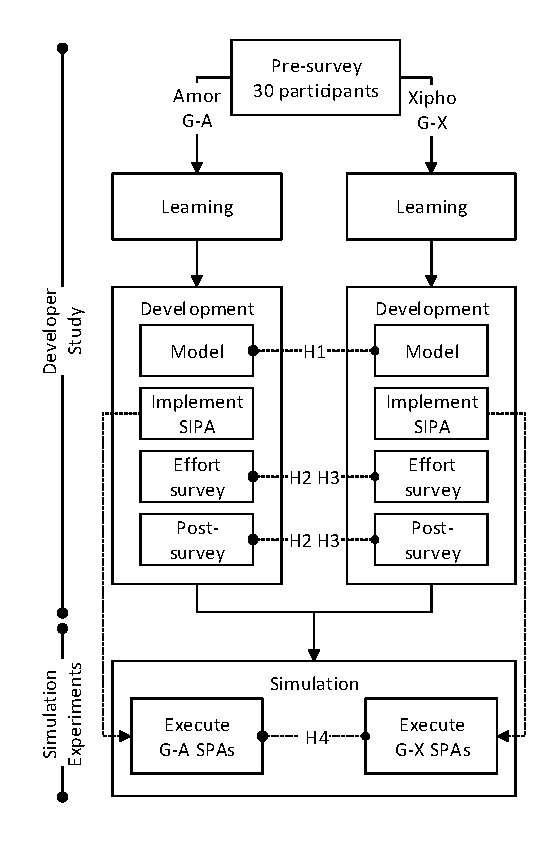
\includegraphics[angle=0,width={0.60\columnwidth}]{Chapter-3/fig/design}
\caption[Experimental design]{Experimental design.}
\label{fig:design} \end{figure}

\subsubsection*{Study Unit} 

The study unit is a ringer manager SIPA discussed 
in Examples~\ref{ex:ringer-meeting}--\ref{ex:ringer-accident} and Figure~\ref{fig:xipho-ringer-as-is}.

\subsubsection*{Participants}

The developer study involved 30 participants, enrolled in a
graduate-level computer science course. The participants earned points
toward their course grades for completing the tasks described. However,
participation in the study was not mandatory. Nonparticipants were
offered an alternative task to earn points equivalent to what they would
earn by participating in the study.

\subsubsection*{Study Mechanics}

This developer study has two phases: learning and development.  The study 
follows the one-factor design with two alternatives (\frameworkA and Xipho).  
We use Xipho as our baseline method because it is best suited among the
existing AOSE methods to engineer personal agents.

We split participants into two groups (A that follows \frameworkA, and X
that follows Xipho) balanced on skills indicated in a presurvey
(detailed in Appendix~\ref{appsec:presurvey}). All participants develop
a ringer manager SIPA.

\begin{description}[leftmargin=1em]

\item[Learning Phase.] During the learning phase of the study,
participants proposed a SIPA, and created models of the proposed SIPA.
This phase sought to help participants understand the nuances of a SIPA,
and to teach them how to model requirements. The data collected in the
learning phase is not used in the evaluation. 

\item[Development Phase.] In the development phase, participants
modeled and implemented a ringer manager SIPA that adapts according
to expectations of callers and 
neighbors, and sanctions received from callers and
neighbors for each action.

\end{description}

In the two development phases, participants were provided with a testbed
to verify the working of their SIPAs.

\subsubsection*{Deliverables}

The participants submitted models and source code at the completion of
the development phase. Additionally, the participants completed a time
and effort survey (detailed in Appendix~\ref{appsec:effortsurvey}) for
each work session, and completed a post-phase survey (detailed in
Appendix~\ref{appsec:postsurvey}) at the end of each phase.

\subsubsection*{Metrics}

To measure the effectiveness of \frameworkA, we compute the following metrics.

\begin{description}[leftmargin=1em]
\item[Model coverage] measures the completeness of the model. It is the
ratio of the number of requirements identified correctly in the produced
model to the total number of requirements of the SIPA. Higher is better.

\item[Model correctness] measures how correct the model is.  It is the
ratio of the number of correctly identified requirements to the total
number of requirements of the SIPA identified.  Higher is better.

\item[Model quality] is the product of model coverage and model
correctness. Higher is better.

\item[Time to develop] is the actual time spent by participants in hours
to develop the SIPA.  Lower is better.

\item[Difficulty of development] is the subjective rating by
participants on how easy it is to develop the SIPA on a Likert scale of
1 (very easy) to 7 (very difficult). Lower is better.

\item[Effort to develop] is the product of time spent in hours and ease
of development rating for each work session. Lower is better.
\end{description}

\subsubsection*{Hypotheses}

We consider the following hypotheses.

\bhypothesis

\item Developers who follow \frameworkA produce better quality models 
than those who follow Xipho.  

\item Developers who follow \frameworkA spend less time to develop 
a SIPA, than those who follow Xipho.

\item Developers who follow \frameworkA feel it is easier to develop 
a SIPA, than those who follow Xipho.

\item Developers who follow \frameworkA expend less effort to develop 
a SIPA, than those who follow Xipho.

\ehypothesis

\subsubsection*{Threats and Mitigation}

We mitigated three main threats to our studies. Differences amongst
participants' programming and modeling skills are inevitable. To handle
the skill differences between participants, we surveyed participants
about their educational backgrounds and prior experiences with
programming and conceptual modeling. We balanced the two groups based on
the survey. To mitigate the risk of participants' failing to report information,
participants were instructed to complete a time and effort survey after
each work session, while it was fresh in their minds. Communication
between participants of different groups is yet another threat. To
mitigate the risk of contamination, we created separate message boards for each
participant group, and restricted participants to only posting
clarification questions on the group message boards.



\subsection{Simulation Experiments}
\label{sec:arnor-simulation}

We further investigate our research question via simulation experiments.
We execute the ringer manager SIPAs implemented by third-party
developers (as part of the aforementioned developer study) on a testbed
fabricated to simulate different real-world environments.


\subsubsection*{Ringer adaptation scenarios}

To test runtime adaptability, we test the applications for
multiple iterations of incoming phone calls during a meeting.

\begin{description}[leftmargin=1em]
\item[Norms fixed.] 
The meeting room participants are committed to keeping their 
phones silent.

\item[Change in norms.] 
The meeting room participants are initially committed to keeping their
phones silent, but later the commitment expires. 

\item[Change in context.] 
The meeting room participants are always committed to keeping their
phones silent. Initially there are several participants in the meeting, but later
all but two leave the meeting.

\item[Change in sanction.] 
The meeting room participants are always committed to keeping their 
phones silent. Initially they give negative feedbacks for loud ringing
but later give more neutral feedbacks. 
\end{description}


\subsubsection*{Metrics}

To measure social experience, we compute the following social metrics
in each of the above adaptation scenarios. 
\begin{description}[leftmargin=1em] 
\item[Adaptability coverage] measures the completeness of code for
adaptability requirements. It is the ratio of the number of adaptability
requirements implemented correctly to the total number of adaptability
requirements. Higher is better.

\item[Adaptability correctness] measures the correctness of the code for
adaptability requirements. It is the ratio of the number of correctly 
implemented adaptability requirements to the total number of adaptability
requirements implemented. Higher is better.

\item[Norm compliance] refers to the proportion of norm instances that
are satisfied. Higher is better.

\item[Sanction proportion] measures the percentage of sanctions imposed.
Lower is better.
\end{description}

\subsubsection*{Hypotheses}

We consider these additional hypotheses:

\bhypothesis

\item SIPAs developed using \frameworkA yields better adaptability
than SIPAs developed using Xipho.

\item SIPAs developed using \frameworkA provide a richer social
experience than SIPAs developed using Xipho.

\ehypothesis

We use adaptability coverage and correctness to test hypothesis
H$_5$, and use norm compliance and sanction proportion measures to test
hypothesis H$_6$.

\section{Results}
\label{sec:arnor-result}

We analyze deliverables produced by participants at the end of each
phase, and compute the study parameters for each deliverable.  

\subsection{Developer Study}

To test hypothesis H$_1$, we compare the models produced by Groups A and X.
For hypothesis H$_2$, we compare the development time expended by
Groups A and X during the two development phases. For
hypothesis H$_3$, we compare the ease of development ratings reported by
Groups A and X during the two development phases, and
for hypothesis H$_4$, we compare their expended effort.

\begin{description}[leftmargin=1em]
\item[Model quality.] We evaluated models produced by the participants 
for correctness and coverage, and computed a quality metric.  We found 
no significant difference in model quality. 

\item[Time and effort to develop.] We found that average time ($13.27$
hours) and effort ($61.54$) expended by the participants using
\frameworkA to be lower than average time ($17.72$ hours) and effort
($96.6$) expended by the participants using Xipho.
Figures~\ref{fig:dev-time} and \ref{fig:dev-effort} show the boxplots
for time and effort expended by participants using \frameworkA and Xipho
to develop the social ringer SIPA.

\begin{figure}[!htb] \centering
  \begin{tikzpicture}
    \tikzstyle{every node}=[font=\small]
    \begin{axis}[
	y=0.7cm,
	ytick={1,2,3,4},
	yticklabel style={align=center},
	yticklabels={Xipho,\frameworkA},
	width=10cm,
	xtick={1,5,10,15,20,25},
	xlabel={Time in hours},
	xlabel style={align=center},
	xmin=0, xmax=30,
	boxplot/average=auto,
	title style={align=center},
	title={Development Time},
	title style={yshift=-1ex,},
	]
	\addplot+[red,boxplot,mark options={fill=red}]
	table[x expr=\coordindex, y index=0]
	{Chapter-3/data/X-dev-time.csv};
	\addplot+[blue,boxplot,mark options={fill=blue}]
	table[x expr=\coordindex, y index=0]
	{Chapter-3/data/A-dev-time.csv};

    \end{axis}
  \end{tikzpicture}
\caption[\frameworkA vs.\ Xipho: Development time]{\frameworkA vs.\ Xipho's development time in hours as reported 
in the work session surveys.}
\label{fig:dev-time}
\end{figure}

\item[Difficulty of development.] The participants using \frameworkA 
found it easier to develop SIPAs with \frameworkA, compared to
participants using Xipho. Figure~\ref{fig:dev-ease} shows the difficulty of
development boxplots.


\begin{figure}[!htb] \centering
  \begin{tikzpicture}
    \tikzstyle{every node}=[font=\small]
    \begin{axis}[
	y=0.7cm,
	ytick={1,2,3,4},
	yticklabel style={align=center},
	yticklabels={Xipho,\frameworkA},
	width=10cm,
	xtick={10,50,100,150},
	xlabel={Effort},
	xmin=0, xmax=160,
	xlabel style={align=center},
	boxplot/average=auto,
	title style={align=center},
	title={Development Effort},
	title style={yshift=-1ex,},
	]
	\addplot+[red,boxplot,mark options={fill=red}]
	table[x expr=\coordindex, y index=0]
	{Chapter-3/data/X-dev-effort.csv};
	\addplot+[blue,boxplot,mark options={fill=blue}]
	table[x expr=\coordindex, y index=0]
	{Chapter-3/data/A-dev-effort.csv};

    \end{axis}
  \end{tikzpicture}
\caption[\frameworkA vs.\ Xipho: Development effort]{\frameworkA vs.\ Xipho's development effort as reported in the work 
session surveys.}
\label{fig:dev-effort}
\end{figure}

\begin{figure}[!htb] \centering
  \begin{tikzpicture}
    \tikzstyle{every node}=[font=\small]
    \begin{axis}[
	y=0.7cm,
	ytick={1,2,3,4},
	yticklabel style={align=center},
	yticklabels={Xipho,\frameworkA},
	width=10cm,
	xtick={1,2,3,4,5,6,7},
	xlabel={},
	xlabel style={align=center},
	xmin=1, xmax=7,
	boxplot/average=auto,
	title style={align=center},
	title={Model},
	title style={yshift=-1ex,},
	]
	\addplot+[red,boxplot,mark options={fill=red}]
	table[x expr=\coordindex, y index=0,col sep=comma]
	{Chapter-3/data/X-dev-ease.csv};
	\addplot+[blue,boxplot,mark options={fill=blue}]
	table[x expr=\coordindex, y index=0,col sep=comma]
	{Chapter-3/data/A-dev-ease.csv};

    \end{axis}
  \end{tikzpicture}

  \vspace{2em}
%

  \begin{tikzpicture}
    \tikzstyle{every node}=[font=\small]
    \begin{axis}[
	y=0.7cm,
	ytick={1,2,3,4},
	yticklabels={Xipho,\frameworkA},
	width=10cm,
	xtick={1,2,3,4,5,6,7},
	xlabel={},
	xlabel style={align=center},
	xmin=1, xmax=7,
	boxplot/average=auto,
	title style={align=center},
	title={Implementation},
	title style={yshift=-1ex,},
	]
	\addplot+[red,boxplot,mark options={fill=red}]
	table[x expr=\coordindex, y index=1,col sep=comma]
	{Chapter-3/data/X-dev-ease.csv};
	\addplot+[blue,boxplot,mark options={fill=blue}]
	table[x expr=\coordindex, y index=1,col sep=comma]
	{Chapter-3/data/A-dev-ease.csv};

    \end{axis}
  \end{tikzpicture}

  \vspace{2em}
%

  \begin{tikzpicture}
    \tikzstyle{every node}=[font=\small]
    \begin{axis}[
	y=0.7cm,
	ytick={1,2,3,4},
	yticklabels={Xipho,\frameworkA},
	width=10cm,
	xtick={1,2,3,4,5,6,7},
	xlabel={},
	xlabel style={align=center},
	xmin=1, xmax=7,
	boxplot/average=auto,
	title style={align=center},
	title={Testing},
	title style={yshift=-1ex,},
	]
	\addplot+[red,boxplot,mark options={fill=red}]
	table[x expr=\coordindex, y index=2,col sep=comma]
	{Chapter-3/data/X-dev-ease.csv};
	\addplot+[blue,boxplot,mark options={fill=blue}]
	table[x expr=\coordindex, y index=2,col sep=comma]
	{Chapter-3/data/A-dev-ease.csv};

    \end{axis}
  \end{tikzpicture}

\caption[\frameworkA vs.\ Xipho: Difficulty of development]{\frameworkA vs.\ Xipho's difficulty of development on a Likert scale of 1 (very easy) to 7 (very difficult).}
\label{fig:dev-ease}
\end{figure}

\end{description}

\subsection{Simulation Experiments}

To evaluate H$_5$ and H$_6$, we analyzed the SIPA's implementation code
and executed the SIPAs in diverse scenarios. We compare the execution
results of \frameworkA and Xipho groups.

\begin{description}[leftmargin=1em]

\item[Adaptability features.] We found average adaptability coverage
($80$\%) to be the same for SIPAs developed by the \frameworkA and Xipho
groups. This result could be attributed to the limited time we gave the
participants to develop the SIPA. Average adaptability correctness was
found to be higher for \frameworkA ($100$\%) compared to the Xipho
($95$\%). This gain could be attributed to the systematic steps provided
by \frameworkA to engineer SIPAs.

\item[Norm compliance.]  Figure~\ref{fig:simulation-compliance} shows 
line plots for norm compliance in the four ringer adaptation scenarios. Though 
the average norm compliance values for SIPAs developed using \frameworkA and Xipho 
are mostly similar, \frameworkA performs slightly better in the fixed norms scenario. 

\begin{figure}[!tb]
    \centering
    \begin{tikzpicture}
    \begin{axis}[
        title={Norms fixed},
        height=7cm,
        width=7cm,
        xlabel={Time tick},
        ylabel={Norm Compliance \%},
        xmin=1, xmax=10,
        ymin=0, ymax=100,
        xtick={1,2,3,4,5,6,7,8,9,10},
        legend pos=north west,
        legend style={font=\small},
        ymajorgrids=true,
        grid style=dashed,
        ]

        \addplot table [x=tick, y=percentage, col sep=comma] {Chapter-3/data/A-compliance-1.csv};
        \addplot table [x=tick, y=percentage, col sep=comma] {Chapter-3/data/X-compliance-1.csv};
        \legend{\frameworkA,Xipho}

    \end{axis}
  
    \end{tikzpicture}
    \hspace{2em}
    \begin{tikzpicture}
    \begin{axis}[
        title={Change in norms},
        height=7cm,
        width=7cm,
        xlabel={Time tick},
        %ylabel={Norm Compliance \%},
        xmin=1, xmax=10,
        ymin=0, ymax=100,
        xtick={1,2,3,4,5,6,7,8,9,10},
        yticklabel=\empty,
        legend pos=north west,
        legend style={font=\small},
        ymajorgrids=true,
        grid style=dashed,
        ]

        \addplot table [x=tick, y=percentage, col sep=comma] {Chapter-3/data/A-compliance-2.csv};
        \addplot table [x=tick, y=percentage, col sep=comma] {Chapter-3/data/X-compliance-2.csv};
        \addplot +[mark=none,dashed] coordinates {(5, 0) (5, 100)};
        \legend{\frameworkA,Xipho}

    \end{axis}
    
    \end{tikzpicture}
    
    \vspace{2em}

    \begin{tikzpicture}
    \begin{axis}[
        title={Change in context},
        height=7cm,
        width=7cm,
        xlabel={Time tick},
        ylabel={Norm Compliance \%},
        xmin=1, xmax=10,
        ymin=0, ymax=100,
        xtick={1,2,3,4,5,6,7,8,9,10},
        legend pos=north west,
        legend style={font=\small},
        ymajorgrids=true,
        grid style=dashed,
        ]

        \addplot table [x=tick, y=percentage, col sep=comma] {Chapter-3/data/A-compliance-3.csv};
        \addplot table [x=tick, y=percentage, col sep=comma] {Chapter-3/data/X-compliance-3.csv};
        \addplot +[mark=none,dashed] coordinates {(5, 0) (5, 100)};
        \legend{\frameworkA,Xipho}

    \end{axis}
    
    \end{tikzpicture}
    \hspace{2em}
    \begin{tikzpicture}
    \begin{axis}[
        title={Change in sanction},
        height=7cm,
        width=7cm,
        xlabel={Time tick},
        %ylabel={Norm Compliance \%},
        xmin=1, xmax=10,
        ymin=0, ymax=100,
        xtick={1,2,3,4,5,6,7,8,9,10},
        yticklabel=\empty,
        legend pos=north west,
        legend style={font=\small},
        ymajorgrids=true,
        grid style=dashed,
        ]

        \addplot table [x=tick, y=percentage, col sep=comma] {Chapter-3/data/A-compliance-4.csv};
        \addplot table [x=tick, y=percentage, col sep=comma] {Chapter-3/data/X-compliance-4.csv};
        \addplot +[mark=none,dashed] coordinates {(5, 0) (5, 100)};
        \legend{\frameworkA,Xipho}

    \end{axis}
    
    \end{tikzpicture}
    \caption[\frameworkA vs.\ Xipho: Norm compliance]{\frameworkA vs.\ Xipho's norm compliance.}
    \label{fig:simulation-compliance}
\end{figure}

\item[Sanction proportion.] Figure~\ref{fig:simulation-sanction-count}
shows the plots for sanction proportion in the four adaptation scenarios.
For the first three scenarios (norms fixed, norms change, and
context change), the SIPAs developed using \frameworkA have a lower
sanction proportion. For the sanction change adaptation scenario, the SIPAs
developed using \frameworkA take slightly longer to adapt, and only have
a slightly higher sanction proportion than the SIPAs developed using Xipho.

\begin{figure}[!tb]
    \centering
    \begin{tikzpicture}
    \begin{axis}[
        title={Norms fixed},
        height=7cm,
        width=7cm,
        xlabel={Time tick},
        ylabel={Sanction \%},
        xmin=1, xmax=10,
        ymin=0, ymax=100,
        xtick={1,2,3,4,5,6,7,8,9,10},
        legend pos=south west,
        legend style={font=\small},
        ymajorgrids=true,
        grid style=dashed,
        ]

        \addplot table [x=tick, y=percentage, col sep=comma] {Chapter-3/data/A-sanction-1.csv};
        \addplot table [x=tick, y=percentage, col sep=comma] {Chapter-3/data/X-sanction-1.csv};
        \legend{\frameworkA,Xipho}

    \end{axis}
    
    \end{tikzpicture}
  \hspace{2em}
    \begin{tikzpicture}
    \begin{axis}[
        title={Change in norms},
        height=7cm,
        width=7cm,
        xlabel={Time tick},
        xmin=1, xmax=10,
        ymin=0, ymax=100,
        xtick={1,2,3,4,5,6,7,8,9,10},
        yticklabel=\empty,
        legend pos=south west,
        legend style={font=\small},
        ymajorgrids=true,
        grid style=dashed,
        ]

        \addplot table [x=tick, y=percentage, col sep=comma] {Chapter-3/data/A-sanction-2.csv};
        \addplot table [x=tick, y=percentage, col sep=comma] {Chapter-3/data/X-sanction-2.csv};
        \addplot +[mark=none,dashed] coordinates {(5, 0) (5, 100)};
        \legend{\frameworkA,Xipho}

    \end{axis}
    
    \end{tikzpicture}

    \vspace{2em}

    \begin{tikzpicture}
    \begin{axis}[
        title={Change in context},
        height=7cm,
        width=7cm,
        xlabel={Time tick},
        ylabel={Sanction \%},
        xmin=1, xmax=10,
        ymin=0, ymax=100,
        xtick={1,2,3,4,5,6,7,8,9,10},
        legend pos=south west,
        legend style={font=\small},
        ymajorgrids=true,
        grid style=dashed,
        ]

        \addplot table [x=tick, y=percentage, col sep=comma] {Chapter-3/data/A-sanction-3.csv};
        \addplot table [x=tick, y=percentage, col sep=comma] {Chapter-3/data/X-sanction-3.csv};
        \addplot +[mark=none,dashed] coordinates {(5, 0) (5, 100)};
        \legend{\frameworkA,Xipho}

    \end{axis}
    
    \end{tikzpicture}
  \hspace{2em}
    \begin{tikzpicture}
    \begin{axis}[
        title={Change in sanction},
        height=7cm,
        width=7cm,
        xlabel={Time tick},
        xmin=1, xmax=10,
        ymin=0, ymax=100,
        xtick={1,2,3,4,5,6,7,8,9,10},
        yticklabel=\empty,
        legend pos=south west,
        legend style={font=\small},
        ymajorgrids=true,
        grid style=dashed,
        ]

        \addplot table [x=tick, y=percentage, col sep=comma] {Chapter-3/data/A-sanction-4.csv};
        \addplot table [x=tick, y=percentage, col sep=comma] {Chapter-3/data/X-sanction-4.csv};
        \addplot +[mark=none,dashed] coordinates {(5, 0) (5, 100)};
        \legend{\frameworkA,Xipho}

    \end{axis}
    \end{tikzpicture}
    \caption[\frameworkA vs.\ Xipho: Sanction proportion]{\frameworkA vs.\ Xipho's sanction proportion.}
    \label{fig:simulation-sanction-count}
\end{figure}

\end{description}

\subsection{Threats to Validity}
\label{sec:threats-to-validity}

In the developer study, we mitigated the threats of skills difference,
participants' failure to report information, and the risk of
contamination. However, some threats remain.

First, our results are based only on the development of a single SIPA
(ringer). For conclusive results on the effectiveness of \frameworkA,
future studies may require participants to develop more than one kind of
SIPA.

Second, the SIPAs developed by the study participants mostly reflect the
participants' (developers) privacy attitudes and information sharing
preferences. To generalize our results, it is required to collect real
data on SIPA users' privacy attitudes and information sharing
preferences.

Third, in simulation experiments, we tested runtime adaptability of
SIPAs under diverse, but a limited set of scenarios. The scenarios we
incorporated may not represent all real world scenarios in which a
ringer SIPA would be employed.

Collecting real data about users' attitudes, preferences, and contexts
is essential, though nontrivial, to mitigate the second and third
threat. Crowdsourcing is a promising avenue for future studies to
collect such data at a large scale.

\section{Related Works}
\label{sec:arnor-related}

\citet{Ali-2013-Reasoning} propose an AOSE-based contextual 
requirements engineering framework, with a focus on consistency and
conflict analysis.  \frameworkA goes beyond conflict analysis, and 
promotes goals, plans, and norms that promote greater social experience. 
\citet{Rahwan-2006-Integrating} propose a framework
to integrate goal models and social models. \frameworkA models subsume
social models, and provide richer abstractions to capture agents'
interactions and affects on experience. 

\citet{Sugawara-IJCAI11-Emergence} attempt to resolve
conflicts through reinforcement learning. \citet{Mashayekhi-IJCAI16-Silk} propose a hybrid mechanism to monitor
interactions and recommend norms to resolve conflicts. 
\citet{Mihaylov-2014-Decentralized} study convergence and propose a
decentralized approach based on strategies in game theory. 
\citet{Villatoro-TAAS13-Robust} introduce social instruments to
facilitate norm emergence via social learning. 
\citet{Yu-AAMAS13-Emergence} study norm emergence through collective
learning from local interactions, and find that collective learning is
superior to pairwise learning. \frameworkA provides constructs to
engineer socially adaptable SIPAs that can make use of these approaches
for norm emergence.

\citet{Hao-FSE16-Norms+formal} propose a lightweight formal
method to design normative systems, which uses Alloy modeling language
and analyzer to synthesize and refine norms. 
\Citet{vanRiemsdijk-AAMAS15-SociallyAdaptive} propose a semantic norm
compliance framework for socially adaptive agents. They use LTL to
express norms. Agents in van Riemsdijk {\etal}'s framework identify and
adopt new norms, and determine execution mechanisms to comply to these
norms. \citet{Aldewereld-TAAS16-GroupNorms} present a
formalism for group norms, and provide mechanisms to reason about these
norms. \citet{Ajmeri-IJCAI16-Coco} propose Coco, a
formalism to express and reason about conflicting commitment instances
at runtime, and dominance among them. Coco employs Answer Set
Programming to compute the nondominated commitment instances and
determines compliance of actions with nondominated commitment instances.
These formalisms could use \frameworkA's social constructs to assist
SIPAs in compliance, adoption of new norm, and resolution of conflicts
amongst norms at runtime.

\section{Conclusion and Future Directions}
\label{sec:arnor-discussion}

We advance the science of privacy by tackling nuanced notions of
privacy, including intrusion, disapprobation, and information leakage,
in personal agents. We treat respecting stakeholders' privacy as an
inherent aspect of delivering a social experience. We envision socially
intelligent personal agents that
\begin{enumerate*}[label=(\arabic*)]
\item adapt to the social contexts of their stakeholders; and
\item act and interact in their best interest (not just the primary stakeholder).  
\end{enumerate*}

We develop \frameworkA, a method that provides social constructs to
engineer privacy-aware social agents. We demonstrate the method via a
ringer manager SIPA. We evaluate \frameworkA using a developer study and
simulation experiments. Compared to Xipho, we find that \frameworkA
\begin{enumerate*}[label=(\arabic*)]
\item facilitates faster development of SIPAs; and
\item yields SIPAs of higher quality, higher adaptability correctness, 
lower sanction proportion, and similar adaptability coverage and norm compliance.
\end{enumerate*}
These observations suggest that \frameworkA promotes SIPAs to deliver a rich 
social experience.

\subsection*{Future Directions}

\citet{Ferreira-AAAI13-GroupRelations} propose a
computational model for emotional agents that considers norms, social
relations, roles and socially acceptable behaviors in a given context.
\citet{Sollenberger-AAMAS11-Kokomo} introduce Kokomo 
to develop affective applications, and provide a middleware for building 
such applications. 
Incorporating an affective \citep{Sollenberger-AAMAS11-Kokomo} and emotional
basis of norms in social agents is an interesting future direction.
Modeling affect could assist SIPAs learn contextually relevant norms. 
A middleware implementation of \frameworkA could facilitate development.

\citet{TOCHI-17:Multiuser} study how context, users' preferences, 
and arguments influence a sharing decision in a multiuser privacy scenario. 
They collect data about appropriate sharing policies for a variety of multiuser
scenarios from human participants in a large scale study. We conjecture that 
such data can be used to seed SIPAs with an initial set of norms, which the 
SIPAs can evolve once put to use.
